\documentclass[a5paper,titlepage,11pt,openany]{scrbook}
\usepackage[a5paper,backref]{hyperref}
\usepackage[papersize={148.5mm,215mm},twoside,bindingoffset=0.5cm,hmargin={2cm,2cm},
				vmargin={2cm,2cm},footskip=1.1cm,driver=dvipdfm]{geometry}
\usepackage{palatino}
\usepackage[utf8]{inputenc}

\usepackage{pstricks}
\usepackage{graphicx}
\usepackage[bahasa]{babel} 
\usepackage{lettrine}
\usepackage{pifont}
\usepackage{enumitem}
\usepackage{wrapfig}
\usepackage{indentfirst}
\usepackage{parcolumns}
\usepackage[titles]{tocloft}
\usepackage{longtable}
\usepackage{microtype}
\usepackage{hyphenat}
%\usepackage[raggedright]{titlesec}
%\usepackage{titletoc}


\renewcommand{\cftchapfont}{%
  \fontsize{9}{8}\selectfont
}

\makeatletter
\renewcommand{\@pnumwidth}{1em} 
\renewcommand{\@tocrmarg}{1em}
\makeatother

\author{Lingkungan St. Petrus Maguwo}
\title{Warta Iman}
\setlength{\parindent}{1cm}
\psset{unit=1mm}


\begin{document}
\thispagestyle{empty}
\thispagestyle{empty}
\newcommand{\edisi}[1]{%
\DeclareFixedFont{\PT}{T1}{ppl}{b}{}{0.7in}
\DeclareFixedFont{\PTit}{T1}{ppl}{b}{it}{0.7in}
\DeclareFixedFont{\PTsmall}{T1}{ppl}{b}{it}{0.25in}
\DeclareFixedFont{\PTsmaller}{T1}{ppl}{b}{it}{0.175in}
\DeclareFixedFont{\PTsmallest}{T1}{ppl}{b}{it}{0.15in}

\begin{pspicture}(14cm,2cm)
\rput[rb](10.35cm,3cm){\PTsmallest {#1}}
\rput[lb](-2cm,1.5cm){\PT {WARTA IMAN}}
\rput[lb](0cm,0.5cm){\PTsmall {Lingkungan St. Petrus Maguwo}}
\end{pspicture}%
}

\newcounter{kgkcounter}[chapter]
\renewcommand{\thekgkcounter}{\arabic{kgkcounter}. }
\newcommand{\kgk}[1]{\refstepcounter{kgkcounter}\textbf{\flushleft \textbf{\thekgkcounter #1}}\\}

\newcommand{\kutipan}[1]{%
\noindent{\framebox{\parbox{10cm}{\centering\emph{#1}}}}}

\edisi{November 2011}

%\vspace{1cm}

\begin{center}
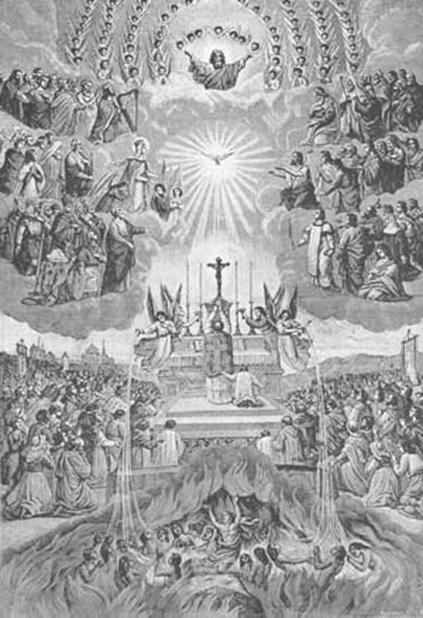
\includegraphics[scale=0.85]{gambar/purgatory2.jpg}
\end{center}

%\vspace{1cm}

\begin{center}
{\PTsmaller {Kasih, kerendahan hati, dan menurut pada kehendak Allah }}
\end{center}

\setlength{\parindent}{1cm}
\pagestyle{plain}
\chap{OMK  St. Petrus  Maguwo\\
 Siap Menjadi Bagian Harapan Gereja}
 
 
       OMK Ya! adalah mereka yang sudah dibaptis dalam Gereja Katolik berusia antara 13 – 35 tahun, belum menikah, aktif atau tidak aktif, berada dalam lingkup teritorial paroki, (stasi, wilayah, lingkungan) ataupun masih dalam lingkup teritorial paroki tetapi berada dalam satu wadah kategorial seperti Legio Maria, Choice, Kharismatik Katolik, Misdinar atau juga di luar kedua lingkup dan wadah itu seperti Pemuda Katolik, PMKRI dan lain sebagainya. Inilah OMK yaitu orang muda katolik yang menyatu dalam satu iman tetapi berada dalam lingkup dan wadah berbeda.
 
     Belum ada data resmi untuk tahun 2012 ini berapa jumlah OMK di Indonesia. Tetapi diperkirakan  hampir 60\% dari jumlah seluruh umat Katolik yang ada di Indonesia adalah OMK. Di lingkungan St. Petrus sendiri berdasarkan buku Informasi Lingkungan yang diterbitkan  tahun 2012 ini, jumlah OMK ada 44 orang, suatu jumlah yang relatif kecil sekitar 20\% dari jumlah umat yang ada 201 orang. Akan tetapi jumlah ini bisa  dipandang cukup sebagai jumlah yang lumayan untuk ukuran suatu lingkungan atau jumlah yang cukup juga untuk suatu keberadaan organisasi yang bersifat kewilayahan/stasi. Sebagai kelompok yang besar sudah barang tentu OMK menjadi tumpuan dan harapan Gereja Katolik Indonesia di masa depan. Dalam konteks inilah OMK khususnya OMK kita Lingkungan St. Petrus harus bisa memposisikan diri untuk siap mengambil bagian dari harapan Gereja itu.
 
\section*{Harapan Gereja Terhadap OMK}
 
      Dalam Temu Raya OMK Keuskupan Agung Semarang yang mengangkat tema “\textit{Tunjukkanlah Merahmu, Buktikanlah Putihmu 100\% Katolik, 100\% Indonesia}” yang berlangsung di Kanisius Yogyakarta 21 Agustus 2011 Bp. Uskup Agung Yohannes Pujasumarto  mengharapkan OMK menjadi orang yang rela berkorban bagi nusa dan bangsa seperti telah dilakukan oleh para pahlawan kita Agustinus Adisutjipto dan Ignatius Slamet Riyadi. Sisi lain OMK hendaknya juga - ini yang utama dan pertama - meneladani Yesus, orang muda yang berdarah-darah dan mati muda untuk menyelamatkan seluruh bangsa. Dengan kata lain Bp. Uskup mau mengatakan pentingnya OMK memiliki keterlibatan penuh bagi keselamatan Republik Indonesia, namun sekaligus mengingatkan pentingya OMK  hidup dan dihidupi oleh iman akan Yesus Kristus  sebagaimana itu dinyatakan dalam tema World Youth Day di Madrid Spanyol 16 -21 Agustus  2011. “\textit{Berakar dalam Kristus dan Dibangun atas Dia, hendaklah Bertambah Teguh dalam Iman” (Kol.2:7)} (pujasumarta.multiply.com)
     
      Hal yang sama juga dikumandangkan oleh Komisi Kepemudaan KWI dengan akan diselenggarakannya Indonesian Youth Day (IYD) 2012 di Sanggau, Kalimantan Barat, 20 - 26 Oktober 2012 mendatang dengan mengusung tema “\textit{Berakar dan Dibangun dalam Yesus Kristus, Berteguh dalam Iman}” dan sub tema “\textit{OMK Makin Beriman, Makin Meng-Indonesia}”. Menurut  Ketua Umum Panitia IYD 2012 dan juga menjabat sebagai Sekretaris Komisi Kepemudaan KWI Romo Yohanes Dwi Harsanto Pr, yang akrab disapa Romo Santo, tema ini mau menegaskan pentingnya OMK memiliki semangat hidup meng-Gereja dengan penghayatan iman yang mendalam. IYD 2012 ingin membawa Kristus kepada OMK dan membawa OMK kepada Kristus sekaligus menyadarkan tugas perutusannya bahwa OMK penting bagi Indonesia dan Indonesia penting bagi OMK.  
\small\textit{(hope-komkepbanjarmasin.blogspot.com)}\normalsize
 
        Harapan besar Gereja Indonesia yang sedang dan telah menggelinding pada tingkat keuskupan dan nasional ini – tentu juga banyak paroki – sesungguhnya selain menunjukkan betapa besar perhatian Gereja terhadap OMK, juga karena  didasari keprihatinan Gereja terhadap bangsa kita yang makin rusak dalam berbagai bidang kehidupan. Melalui beberapa Surat Kegembalaan Prapaskah (SKP) dan Nota Pastoral (NP)  yang dikeluarkan KWI dalam kurun waktu 1997 hingga 2006 Gereja senantiasa mengingatkan  bangsa Indonesia bahwa  bangsa kita sedang bergerak menuju kerusakan moral yang luar biasa (SKP 1997 \& 2001). Bila hal ini terus berlangsung maka kehancuran keadaban publik tak akan terhindarkan lagi. Pada gilirannya kesejahteraan bangsa juga tidak tercapai (NP 2003). Gereja katolik sebagai Gereja yang bercirikan 100\% katolik dan 100\% Indonesia terpanggil untuk ikut serta memperbaiki bangsa dan  mencita-citakan bangsa ini segera memiliki habitus baru terutama habitus baru dalam tata ekonomi yang berkeadilan. Akan tetapi hingga sekarang situasi bangsa tidak beranjak menjadi lebih baik bahkan lebih buruk (NP 2004 \& 2006).
 
       Dalam kerangka itulah Gereja Katolik mencintai dan memandang penting peran OMK dalam    kehidupan bernegara dan berbangsa serta berharap agar OMK bukan saja menjadi putra-putri Gereja yang beriman baik, tetap juga dengan itu menjadi agen-agen transformatif yang mampu menggerakan perubahan menuju Indonesia yang lebih baik. Gereja Katolik Indonesia ingin agar Gereja ke depan  tidak kehilangan masa depannya sebagaimana telah terjadi di Gereja-Gereja Eropa.  OMK  diharapkan tidak  menjadi bagian problema seperti di Negara-negara Eropa melainkan justru menjadi bagian solutif. Kiranya kita pantas menyambut dengan baik apa yang pernah dikatakan Beato Yohanes Paulus II mengenai perlunya evangelisasi baru bagi kaum muda yang menekankan pentingnya mereka bukan hanya sebagai obyek pastoral tetapi juga sebagai  agen dan rekan dalam melakukan misi Gereja dalam berbagai karya kerasulan dalam pelayanan dan cinta (\textit{Eclessia in Asia,} 47).
 
        Kiranya jelas dengan memperhatikan tema-tema yang diusung dalam berbagai pertemuan baik pada tingkat paroki, keuskupan atau pun nanti pada tingkat nasional,  Gereja mengharapkan OMK menjadi komunitas Gereja muda terdepan yang tangguh baik dalam kehidupan beriman maupun dalam tugas perutusannya bagi dan dalam kehidupan bermasyarakat dan berbangsa terutama untuk menanggapi situasi bangsa yang saat ini sedang mengalamai carut-marut menuju kehancuran peradaban.
 
       OMK Lingkungan St. Petrus sebagai bagian dari OMK Indonesia hendaknya memahami dan menyadari betul  harapan Gereja Katolik saat ini. Partisipasi Gereja Katolik Indonesia untuk menyelamatkan bangsa dan negara dari kehancuran peradaban dan membangun Gereja masa depan akan sangat tergantung dari peran aktif OMK sendiri dalam menanggapi harapan Gereja itu. Kita percaya harapan Gereja itu telah menjadi benih yang tertanam dalam hati setiap OMK Lingkungan St. Petrus Maguwo yang siap tumbuh dan berkembang dalam setiap usaha yang telah dan hendak dilakukan.
 
\section*{Spiritualitas Kaum Muda Katolik}
 
      Salah satu ciri utama OMK yang tidak bisa tidak harus ada adalah iman akan Kristus. Ciri yang lain tidak mempunyai daya ikat sekuat iman bahkan tanpa dengannya OMK tidak bisa ada apalagi hidup. Iman menentukan eksistensi OMK. Kekatolikan yang menyatukan pribadi-pribadi OMK satu dengan yang lain adalah wujud kesetiaan pada iman itu. Jadi iman akan Kristus adalah roh yang menjiwai OMK. Roh itu juga yang menggerakkan dan menuntun OMK menggapai harapan dan cita-cita Gereja. Oleh sebab itu OMK harus terus menerus menggeluti imannya agar lebih mendalam dan tangguh dalam segala situasi.
 
       Iman adalah proses terus menerus menanggapi panggilan Allah yang  kasihNya kepada kita nyata dalam hidup Yesus Kristus dan RohNya. Iman adalah jawaban kita atas kasih itu yang mewujud bukan hanya dalam perayaan liturgi, tetapi terlebih dalam hidup sehari-hari. Persoalan-persoalan sosial termasuk persoalan bangsa yang kita hadapi adalah medan bagi perwujudan iman itu. Oleh karena itu iman sebagai bentuk tanggapan atas panggilan atau kasih Allah kepada kita harus kita hayati dalam dialog terus menerus dengan Allah melalui Kristus dan RohNya. Dalam dialog itu kita akan merasakan bahwa Allah itu ada dan nyata dalam hidup kita, bahwa Allah itu membantu dan melindungi kita serta mendorong kita untuk kuat dan berani menghadapi persoalan hidup bahkan persoalan hidup berbangsa dan bernegara dan dalam semuanya itu tugas perutusan kita sebagai orang katolik atau OMK  menjadi nyata. Inilah spiritualitas OMK yang mengalir dari iman akan Trinitas, Allah Bapa, Allah Putra dan Allah Roh Kudus.
     
      Ada dua model biblis yang bisa menjadi gambaran penghayatan spiritualitas OMK dalam menyikapi soal-soal hidup bersama terutama persoalan bangsa saat ini. Model pertama adalah pengalaman iman Abraham dalam Tuhan dan model kedua adalah perjuangan Musa demi keadilan bagi bangsanya. Kedua model ini memuncak pada perjumpaan dengan Kristus sebagaimana dikatakan dalam Injil Yohanes bahwa Yesus bertemu Abraham dalam sejarah sebab “ sebelum Abraham ada Aku ada” (Yoh. 8:58) Demikian pun Musa sebagaimana ditegaskan dalam surat St. Paulus kepada umat Ibrani “ Karena iman maka Musa setelah dewasa menolak disebut anak puteri Firaun, karena ia lebih suka menderita sengsara dengan umat Allah daripada untuk sementara menikmati kesenangan dari dosa. Ia menganggap penghinaan karena Kristus sebagai kekayaan yang lebih besar dari pada semua harta Mesir sebab pandangannya ia arahkan kepada upah” (Ibr. 11: 24-26)
     
        Dalam sejarah keselamatan, kita mengenal bagaimana Abraham meninggalkan rumah dan keluarganya karena ketaatannya kepada suara batinnya untuk berangkat ke tempat yang tidak jelas baginya. Dengan seluruh penderitaan yang ia alami selama pencarian panjang itu termasuk permintaan mengorbankan puteranya Ishak anak yang dicintai, Abraham memperlihatkan  ketaatan kepada Dia yang menuntunnya ke tempat yang ia belum kenal. Sikap lepas Abraham dalam ketaatannya kepada Tuhan ini akhirnya berujung pada suatu pembentukan bangsa. Inilah suatu perjalanan iman yang dari hari ke hari semakin mendalam hingga akhirnya Tuhan menganugerahi suatu bangsa, suatu buah anugerah iman.
 
      Berbeda dengan Abraham, Musa mengawali perjalanan imannya justru dari realitas kehidupan yaitu dari keterlibatannya kepada bangsanya. Ia tidak mau menjadi bagian dari sistem yang menindas melainkan justru menjadi bagian dari orang yang tertindas. Kesiapan dan ketaatannya kepada cinta yang membebaskan ini Musa akhirnya berjumpa dengan Tuhan ketika ia sampai ke puncak gunung Sinai. Inilah cinta yang berakhir dalam Tuhan.
     
     Dari kedua model biblis pengalaman Musa dan Abraham, kita bisa memahami bahwa penghayatan spiritualitas OMK mendapat bentuknya dalam sinergitas dari kedua model biblis itu. Apa yang didapat dari pengalaman iman (Tuhan) harus berujung pada cinta kepada bangsa Indonesia dan sebaliknya cinta kepada bangsa Indonesia harus berakhir pada cinta kepada Tuhan.   Setiap pribadi OMK  harus menjadi seorang contemplativus simul in actiones sebagaimana St. Ignasius dari Loyola. yaitu seorang yang beriman dan serentak mewujudkan imannya dalam keterlibatanya dalam soal-soal sosial termasuk hidupnya atau persoalan bangsa. Keterlibatan ini bukanlah merupakan semacam penerapan iman melainkan sungguh-sungguh merupakan bagian integral dari seluruh perutusannya sebagai kaum beriman. Seorang pribadi OMK harus siap meninggalkan “ruang Gereja” untuk menggemakan jawabannya kepada Allah dalam persoalan hidup sehari-hari termasuk persoalan bangsa.
 
\section*{Siap dalam Harapan Gereja}                                
 
     Sekarang apa yang baik dilakukan oleh OMK khususnya OMK kita St. Petrus Maguwo? Kita masih ingat apa yang diharapkan oleh Romo Yulius Blasius Fitri Gutanto Pr dalam kotbahnya ketika ia melantik pengurus OMK Lingkungan St. Petrus Maguwo periode 2011 - 2013 di Kaliurang  Wisma Omah Jawi 5 – 6 Maret 2011 bahwa setiap pribadi OMK harus menjadi pribadi beriman yaitu orang katolik sejati, bukan orang katolik KTP. Dalam arti lebih luas apa yang dikatakan Romo mempunyai relevansi jelas bahwa orang katolik sejati adalah orang katolik 100\%, tetapi  juga 100\% orang Indonesia. Kesejatian orang katolik terletak pada kesetiaan  iman dan keterlibatannya kepada persoalan hidup baik persoalan hidup masyarakat,  bangsa dan  negara.
 
      Memposisikan diri sebagai OMK sejati tidak lain adalah OMK yang siap melaksanakan tugas perutusannya seiring dengan derap langkah Gereja Katolik Indonesia saat ini. Akan tetapi kesiapan perutusan demikian tidak berarti menunggu dalam keadaan pasif, tidak berbuat sesuatu,  melainkan justru menunggu dalam keadaaan aktif, seperti digambarkan dalam perumpamaan 10 gadis yang menunggu mempelai datang, lima diantaranya bodoh dan lima bijaksana. (Mat. 25:1 – 13) Lima yang terakhir merupakan gambaran orang yang menunggu dalam keadaan aktif, karena mereka mengerti apa yang dilakukan dalam keadaan atau selama  menunggu mempelai datang, sehingga ketika mempelai datang mereka tidak kehabisan minyak.
 
      Saya yakin OMK Lingkungan St. Petrus tahu apa yang harus dilakukan saat ini  di sini di tempat ini, di tingkat wilayah, stasi, Paroki  dan secara khusus pada tingkat lingkungan kita, sebagai perwujudan diri dari menunggu dalam keadaan aktif. Berbagai program dan cara melakukan kegiatan tentu sudah dibuat atau seharusnya dibuat. Diharapkan program itu berjalan dengan baik, sebab melalui program dan cara bergiat yang berjalan menunjukkan bahwa roh itu atau iman  akan Kristus mewujud dalam pola penghayatan Abraham dan Musa. Hanya soalnya seringkali program kita tidak berjalan dengan baik atau bahkan mungkin gagal. Tidak apa!
     
       Oleh karena itu barangkali program harus dibuat berdasarkan dialog dengan realitas atau situasi atau kebutuhan umat agar lebih realistis dibanding dengan program berdasarkan ide atau gagasan sekalipun baik.dan diperlukan. Dialog dengan orangtua lingkungan misalnya mungkin penting dilakukan untuk menemukan apa yang perlu dan baik bagi lingkungan, sehingga dengan program-programnya OMK mampu menjadi motor penggerak kehidupan lingkungan atau memiliki peran yang siginifikan. Demikian kiranya berlaku juga pada tingkat wilayah, stasi, Paroki, bahkan dengan masyarakat. Model dialog perlu dipilih dan disesuaikan dengan bagaimana OMK mau melakukan dalam bentuknya. Musa menemukan Tuhan karena dialog dan terlibat dengan persoalan bangsa dan Abraham  dialog dengan imannya menemukan  masyarakat bangsa.
 
      Tulisan ini  bukan hendak membahas program OMK, melainkan mau mengingatkan OMK khususnya OMK lingkungan kita bahwa mereka sekarang berada dalam “gerbong” harapan Gereja Katolik yang sedang melaju menuju masa depan dan berpartisipasi dalam usaha-usaha menyelesaikan persoalan bangsa. Lingkungan St. Petrus kiranya  merupakan lini terdepan dari persoalan-persoalan sosial kita dan dari situlah OMK mulai. Inilah panggilan perutusan kaum muda. Inilah kesiapan OMK lingkungan St. Petrus dalam mengambil bagian dari harapan Gereja Katolik Indonesia.
 
      Dengan memahami apa yang diharapkan Gereja Katolik terhadap OMK dan  dengan penghayatan spiritualitas yang mengalir dari Trinitas dalam model penghayatan biblis Abraham dan Musa, OMK kita khususnya OMK Lingkungan St. Petrus diharapkan selalu berada dalam kesiapan tugas perutusannya melalui berbagai program lingkungan yang dibuatnya. Niscaya dengan kesadaran demikian lingkungan St. Petrus dan masyarakat sekitarnya akan menjadi ladang perwujudan iman OMK dan buahnya terasa khususnya bagi umat lingkungan.
 
\sumber{Yogyakarta, 10 Juni 2012,\\
Hari Raya Tubuh dan Darah Kristus\\(AS)}
\begin{center}
%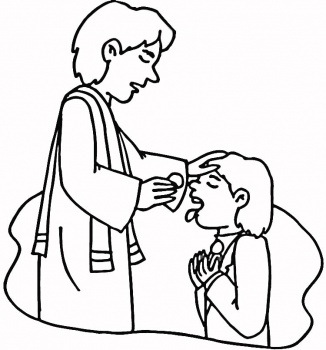
\includegraphics[scale=0.5]{gambar/communion-in-church-coloring-page.jpg}
\end{center}
\chap{Orang Muda Katolik (OMK) dan Liturgi}

\section*{Prasangka}
\small
Dalam praktek, banyak kali muncul masalah pada relasi antara OMK dan liturgi (perayaan iman, ibadat). Di antara liturgi dan OMK seolah ada hubungan ”enggan tapi rindu”. Di balik tema “liturgi dan orang muda”, masih bercokol  prasangka laten baik terhadap Orang Muda Katolik (OMK), maupun terhadap Liturgi Gereja Katolik Roma. OMK seolah-olah suka hura-hura, semaunya sendiri, tidak bisa diatur dalam berliturgi. Sebaliknya, liturgi sering dipandang sebagai aturan sakral dan baku, seakan-akan jauh dari gelora kerinduan orang muda. Terhadap OMK, Tim Liturgi Paroki biasanya mengenakan frasa ”OMK yang pragmatis, maunya serba lain”. Seakan-akan OMK diperlawankan dengan liturgi yang tak memberi ruang kebebasan ungkapan iman. Dari pihak OMK, ada pula prasangka, bahwa liturgi itu serba  kaku.

Prasangka ini  bisa dipahami, karena sifat umum orang muda yang masih dalam masa pertumbuhan yang pesat. Mereka sedang berkembang dalam dimensi psikologis, intelektual, seksual-hormonal, emosi, peran sosial dan iman. OMK memang sedang  mengalami transformasi menuju kepribadian yang integral. Rentang masa muda yang panjang (usia 13-35 th) adalah masa distingtif,  saat mencari, mempertanyakan, belajar dan mengambil keputusan. Kita yang pernah menjalani masa muda tentu merasakan bahwa saat itu merupakan saat yang sukar, menantang sekaligus menggairahkan karena penemuan-penemuan baru. Sering kali kita ingin sesuatu yang ”lain dari pada yang lain” pada masa muda. Sedangkan di pihak lain, Liturgi Gereja Katolik Roma, sudah berkembang dalam 20 abad dan sering dipandang sebagai peraturan yang kaku alih-alih sebagai perayaan yang membebaskan. Padahal, potret berliturgi oleh OMK tak selamanya demikian.

Prasangka dan kecurigaan  yang digeneralisasi begitu saja terhadap OMK itu tentu tidak akan memecahkan persoalan yang sering kali muncul dalam praktek penghayatan OMK terhadap liturgi. Tidak bijaksana,  generalisasi mengenai OMK yang ”pragmatis dan maunya serba lain” itu. Liturgi Gereja pun tidak sepantasnya diperlawankan dengan gejolak dan selera orang muda. Kenyataannya, bahwa banyak orang terpanggil menjadi kudus pada masa muda, dan panggilan kekudusan itu banyak yang bermula dari penghayatan liturgi. Kita pun tahu, Ekaristi Kaum Muda (EKM) baik yang diselenggarakan oleh paroki, maupun oleh Panitia \textit{World Youth Day} yang mendatangkan Sri Paus sebagai pemimpin liturgi, selalu dipenuhi OMK dengan kerinduan mendalam. Bahkan, kelompok misa bahasa Latin yang terkesan ”penuh aturan ketat” ada yang digerakkan  oleh orang muda.

\section*{Memerlukan Dukungan}

Seperti pada umumnya orang Katolik Indonesia, tua maupun muda, penghayatan OMK akan liturgi sebenarnya tergantung pada pengetahuan dan pengalaman mereka akan liturgi itu sendiri. Bahwa praktek liturgi OMK kadang-kadang membuat para penanggungjawab liturgi mengerutkan kening, bagi saya lumrah saja dalam konteks pembelajaran. Gelegak kreativitas masa muda sekaligus tingkat pengetahuan dan pengalaman OMK akan liturgi haruslah bisa dipahami dan didukung. Tak usahlah daya kreatif mereka dalam ber-liturgi dihakimi dengan sewenang-wenang seperti yang sering terdengar dari keluhan mereka. Gara-gara  maunya kreatif, mereka ”dikecam secara liturgis”.

Sepanjang pengalaman para pendamping, tak ada OMK yang menjadi buruk karena mau kreatif dalam merencanakan dan mengolah liturgi. Justeru sebaliknya, para aktivis kelompok-kelompok OMK yang mau proaktif , mau belajar, mau secara jujur mengusulkan berbagai kreasi dalam liturgi, dan karenanya  berani mencari dan melakukan yang benar, berani mengakui  kesalahan bila terjadi dan berani memperbaikinya) terbukti menjadi aktivis  dengan penghayatan liturgi yang nyata dalam perilaku. Lagipula, jika OMK membuat kesalahan dalam ber-liturgi, ternyata kesalahan itu tidaklah fatal, normal saja. Kesalahan mereka pun kadang-kadang karena pengaruh kelompok kategorial  yang lebih senior. Justeru kelompok-kelompok kategorial yang beranggotakan orang-orang tidak muda lagi lah yang sering bikin kesalahan fatal, dan keras kepala, bukan? Sebaliknya, biasanya dengan taat OMK mau belajar dari kesalahan. Mereka tetap gembira dan kreatif, asalkan pendamping dengan empati mau  setia mendampingi, menjelaskan makna simbol dan hakikat liturgi yang kaya makna itu kepada mereka, memetakan posisi kelompok dalam lebensrauung Gereja lokal, dsb. Saya yakin, dalam kerja sama yang baik dengan pendamping itu dapatlah dihindarkan kesalahan-kesalahan fatal yang tidak perlu terjadi. Sebenarnyalah di antara Liturgi dan OMK ada hubungan batin yang saling mendukung. Liturgi menjadi ongoing formation  bagi OMK. Sedangkan daya kreativitas dan gelora kemudaan OMK membuat liturgi dirayakan dengan bersemangat. Liturgi tanpa keterlibatan orang muda, merupakan tanda nyata kematian Gereja.
\normalsize

\section*{Liturgi Kelompok OMK}

Ketika naskah ini diketik (Mei 2008-pen), kantor Youth Desk – FABC di Manila sedang mengolah survei mengenai penghayatan OMK akan Liturgi Ekaristi. Munculnya jajak pendapat untuk OMK mengenai Ekaristi ini didasari praduga bahwa kerinduan OMK akan liturgi berbanding lurus dengan pengetahuan dan pengalaman mereka ber-liturgi.  Tema Liturgi Ekaristi menjadi pembahasan dalam \textit{Asian Youth Day} tahun  2009 di Manila.  Mengapa tema ini diagendakan? Saya menduga, di satu sisi ada kecemasan kalau-kalau  Liturgi  ”ditinggalkan” alias ”tidak laku” lagi di kalangan OMK. Liturgi disangka tidak mampu menjawab kerinduan OMK di tengah arus percepatan globalisasi yang mengasingkan OMK. Di sisi lain ada pula kecemasan kalau-kalau  OMK di berbagai kelompok kategorial yang masih mau aktif ber-liturgi  mulai ”meninggalkan” kaidah liturgi, alias ”mengikuti maunya sendiri”. Komunitas-Komunitas OMK  lebih mementingkan ”rasa kepuasan kelompok” dalam berliturgi dibandingkan ”rasa universal” Gereja. Dua macam kecemasan itu bermuara pada dua pertanyaan atas satu kenyataan liturgi: 
\begin{enumerate}
\item Bagaimanakah liturgi menjawab kerinduan OMK akan perasaan ditemani oleh ”Yang Ilahi” di tengah arus zaman dan perubahan selera ini? \item Bagaimanakan OMK menyadari tanggungjawab dan penghayatannya akan liturgi yang bergairah karena setia pada aturan Gereja?
\end{enumerate}

Saya menemukan dua prasyarat atas jawaban pertanyaan di atas setelah mengamati beberapa komunitas OMK.  Prasyarat itu adalah 
\begin{enumerate}
\item Jika mereka mendapatkan komunitas yang digembalakan dengan semangat berbagi dan mereka dipercaya dalam kegiatan komunitas. 
\item Jika ungkapan kemudaan mereka diberi ruang dan waktu yang cukup dalam liturgi komunitas.
\end{enumerate}

Pada beberapa kelompok OMK, liturgi mereka hayati sepenuh hati. Tampaknya mereka ”puas” dan selalu rindu dengan liturgi komunitas mereka.  Sebabnya, liturgi tak mereka lepaskan  dari kehidupan komunitas kategorial mereka, dan bahwa komunitas memberi ruang dan waktu bagi karakter kemudaan mereka dalam liturgi. Ada ”gembala” (pendamping/ moderator) yang secara tetap mempercayai mereka dalam kegiatan komunitas. Sang pendamping ini (imam dan biarawati/awam) mendampingi liturgi mereka dengan tak bosan mengajarkan prinsip-prinsip  liturgi  sesuai  maksud Gereja. Beberapa kelompok OMK itu adalah: Komunitas Sant’ Egidio (SE), beberapa komunitas Persekutuan Doa Karismatik Katolik (PDKK) muda-mudi, beberapa sel Komunitas  Tritunggal Mahakudus (KTM) muda-mudi; beberapa presidium Legio Mariae (LM) muda-mudi, kelompok Imago Dei (ID), dan kelompok Doa Taize (DT). Mereka memiliki kesamaan pengalaman, bahwa perjumpaan dengan Allah dalam doa, teristimewa liturgi merupakan puncak dan sumber spiritualitas dan kegiatan komunitas.

\section*{Variasi yang Melegakan}

Kelompok-Kelompok OMK itu  biasa berkumpul untuk berdoa secara rutin.  Pertemuan doa mereka mengikuti bukanlah liturgi karena dan karenanya memiliki variasinya masing-masing.  Dalam hal ini Tata Perayaan Sabda atau Ibadat Sabda atau Doa kelompok kategorial di luar Ekaristi, adalah kegiatan non liturgis atau para liturgi atau devosi. Perayaan Sabda adalah liturgi bila dilakukan dalam Ibadat Harian dan liturgi sakramen termasuk Ekaristi yang meliputi dua bagian utama: liturgi Sabda dan Liturgi Ekaristi. Ibadat Sabda di luar liturgi atau para liturgi dan devosi tidak sangat terikat pada kaidah-kaidah liturgi. Dalam hal ini kreativitas orang muda mendapat ruang yang lebih luas dan nyaman. Sebulan atau beberapa bulan sekali mereka mengundang imam untuk merayakan ekaristi. Umumnya, mereka mengikuti aturan liturgi yang baku. KTM dan PDKK  secara berkala membuat adorasi sakramen Mahakudus. Sebaiknya Adorasi Sakramen Mahakudus dibuat sebelum atau sesudah Perayaan Ekaristi, atau sebagai unsur dari Ritus Penutup Ekaristi, dan bukan di tengah liturgi Sabda atau di tengah liturgi Ekaristi.  Beberapa variasi liturgi, khususnya dalam perayaan ekaristi dan adorasi, tampak paling ekstensif dalam PDKK dan KTM.

Lagu-lagu yang dipakai KTM dan PDKK sebagian besar bercorak mirip pop rohani. Ciri khas liturgi PDKK dan KTM adalah sangat ekspresif. Bernyanyi melambungkan pujian kepada Allah, sambil bertepuk tangan, mengangkat tangan, diiringi musik yang meriah. Di sini dikenal juga pencurahan Roh. Salah satu yang khas pula dalam PDKK dan KTM ialah peran pemimpin doa yang mengantar sesi-sesi lagu, doa dan firman. Dalam perayaan ekaristi, ada kesan bahwa peran imam  sebagai pemimpin resmi liturgi Gereja, tenggelam oleh peran pembawa acara yang juga pemimpin doa. Ambil contoh, pengantar tobat yang dibawakan imam, sering kali masih diulang oleh pemimpin doa dengan lebih panjang. Bagaimana hal ini menjadi variasi yang tidak mengganggu? Kuncinya, dialog persiapan antara imam dan pemimpin doa.  Menjadi soal jika imam tidak diajak bicara dahulu  dan celakanya merasa tidak rela karena dilangkahi dalam memimpin doa. Bisa jadi saat homili menjadi saat pelampiasan ketidakpuasan imam. Namun hal ini jarang sekali terjadi dalam kelompok doa OMK. Pemimpin doa komunitas PDKK dan KTM OMK biasanya bisa bekerja sama dengan baik dengan imam pemimpin ekaristi.

Pertemuan doa  DT mendaraskan mazmur dan doa singkat dalam nada sederhana dengan musik lembut dan dekorasi temaram dengan ikon salib Kristus di altar depan. Doa-doa  Sant’ Egidio mirip dengan DT. ”Mereka biasa berdoa sebentar di depan ikon Yesus. Ini sungguh doa inklusif. Pemimpinnya tidak menempatkan diri di depan umat (di belakang altar), tetapi di depan umat. Kalau ada imam ingin berbagi atau memberi keterangan Sabda Tuhan, barulah beliau tampil di mimbar. Hal ini wajar karena pertemuan doa mereka ini bukanlah perayaan Ekaristi.  Sejauh perlu, doa dilakukan “bersama” di depan ikon Yesus. Doa ini juga merupakan relativisasi di hadirat Tuhan. Orang, setelah seharian bekerja, tidak mensyukuri prestasinya atau mengumpat kegagalan hari itu, melainkan mempersembahkan seluruh perjuangan sepanjang hari kepada Tuhan, entah sukses, entah gagal, entah biasa-biasa saja. Sebetulnya cara pandang seperti ini biasa saja. Hanya saja, doa ini dikemas dalam suatu liturgi yang menyentuh hati: di depan ikon besar Yesus, dalam keredupan cahaya gereja, dengan koor satu suara, sederhana, dengan iringan organ, tapi mengantar pada keagungan Tuhan. Liturgi mereka tidak ada yang istimewa. Pengalaman mereka yang selalu dibawa dalam doa-doa harian dan misa di akhir pekan, itulah yang istimewa.

ID mengungkapkan doa bersama sebagai sarana berkomunikasi dengan Tuhan, untuk mengetahui kehendak-Nya, mendapatkan restu, serta mendapat kekuatan. Dasar kegiatan ID ialah saling menguatkan dalam doa (Gal. 6:2; Ef. 6:18-20). Suasana praise and  worship bersifat fun, gembira penuh syukur. Namun jika dilakukan dalam Liturgi (misalnya Ekaristi), apapun bentuk variasi penyesuaian, hendaknya tidak timbul kesan bahwa di tengah liturgi dimasukkkan acara gembira ria yang bersifat profan.  Mereka pun mencari \textit{rhema} untuk minggu itu dan mengungkapkan dalam liturgi.

LM menempatkan devosi kepada Bunda Maria. Namun yang menjadi sentralnya ialah Allah Bapa, Putra dan Roh Kudus.  Semua pusat devosi, ibadat, liturgi adalah Allah: Bapa, Putra dan Roh Kudus. Maka devosi yang khusus kepada Maria itu tidak harus mengaburkan atau menghilangkan sentralnya, tetapi justru semakin mengarahkan para devosan ke sentral: \textit{ad Iesum, ad Patrem, ad Spiritum Sanctum}, itu sebabnya semua orang yang berdoa rosario atau mempunyai devosi khusus kepada Bunda Maria menyalaminya sebagai Putri Allah Bapa, Bunda Allah Putra dan Mempelai Allah Roh Kudus. \textit{Per Mariam ad Iesum}.  Doa  mereka mengikuti tatacara dalam Buku Pegangan LM. Lagu sangat minim, kalaupun ada,  lagu penghormatan kepada Bunda Maria selalu dinyanyikan dengan khusuk. Kerendahan hati dan kesederhanaan menjadi pola doa  kelompok ini. Doa rosario dan \textit{catena legionis} diwajibkan dalam devosi mereka. Jika ada misa, doa rosario dan catena legionis wajib didoakan tetapi sebelum liturgi, sebelum Ekaristi, yang berarti di luar liturgi dan bukan di tengah liturgi. Ini sangat tepat, walaupun mungkin ada yang kurang paham lalu mendoakannya dalam liturgi. Tak banyak OMK yang terlibat dalam LM dibanding kelompok lain.

Walaupun berbeda ungkapan, namun nyatalah bahwa perasaan mereka sama-sama terangkat kepada kehadiran Yang Ilahi dan iman dimantapkan. Adanya penyesuaian dan variasi itu dirasakan melegakan  OMK dalam menghayati iman akan Allah.

\section*{Liturgi yang Tergairahkan oleh Kemudaan}

Apakah istimewanya liturgi orang muda? Sebenarnya tatacara liturgi mereka tidak ada bedanya dengan liturgi pada umunya. Yang istimewa adalah apa yang mereka rindukan dan  cara ungkapannya. Dalam situasi pertumbuhan menuju masa depan yang tidak serba jelas, di tengah zaman yang hiruk pikuk tidak pasti, liturgi menjadi wahana ungkapan mereka. Apakah liturgi bisa menjawab kerinduan mereka? Alih-alih menunggu liturgi memuaskan mereka, maka banyak kali terjadi, mereka-lah yang berinisiatif menggairahkan liturgi sesuai desakan kuat di dalam dada untuk mengungkapkan kerinduan mereka akan Allah. Sayangnya, para penanggungjawab liturgi kadang-kadang tidak (mau) menanggapi dengan sabar. Akibatnya, gairah OMK sering dikecewakan. Yang diperlukan sekarang adalah penanggungjawab liturgi yang melibatkan OMK dalam tim liturgi, agar perencanaan doa-doa dan lagu, serta variasi lain bisa menjawab kerinduan OMK. Ada aneka warna kelompok doa OMK. Sangat bagus jika mereka dilibatkan oleh para penanggungjawab liturgi di berbagai tingkat (paroki, dekenat/kevikepan, dan keuskupan) untuk menggairahkan liturgi kita. Dengan demikian, tak kan ada lagi kecurigaan dan penilaian sepihak atas OMK seperi pada alinea pertama tulisan ini. Mereka pun merasa tersapa dan pasti belajar liturgi Katolik dengan lebih baik. Ada satu lagi potret ber-liturgi OMK walaupun sangat jarang. Yakni OMK yang tergerakkan oleh liturgi sedemikian rupa, sehingga terinspirasi untuk terjun dalam perjuangan menegakkan perdamaian dan keadilan. Mereka pun perlu dilibatkan dalam perencanaan dan pelaksanaan liturgi agar liturgi benar-benar ”puncak dan sumber” hidup beriman bagi OMK.

\section*{OMK dan Musik Liturgi}

Bayangkanlah suatu perayaan Liturgi Ekaristi di gedung gereja yang besar dengan ribuan OMK. Bagaimana jika tanpa musik? Nah, musik ialah salah satu kegemaran favorit OMK, sejak era zaman batu hingga era dot com ini. Namun musik Liturgi, memiliki ketentuan liturgis. Apakah OMK masih tertarik dengan musik liturgi? Atau, apakah musik liturgi masih mampu berdaya pikat terhadap OMK?

Perayaan Liturgi  tidak melulu  pikiran (ratio) . Liturgi selalu meliputi tata gerak dan menyangkut  seluruh kekayaan cita-rasa batin yang mendorong setiap orang untuk mengungkapkannya secara lahir. Wujudnya doa, permohonan, pujian, sembah sujud, dan semacamnya. Relasi dengan Allah ialah misteri. Maka apa pun yang sulit dinyatakan dalam kata-kata, diwujudkan dalam seni yaitu musik, syair, nyanyian, lukisan, pahatan yang menembus misteri relasi Allah dan manusia. Itulah jiwa Liturgi, yaitu Allah yang selalu ingin mengkomunikasikan diri kepada manusia dan manusia yang rindu menyambut-Nya. Ungkapan itu diungkapkan oleh manusia dengan segala dimensi kemanusiaannya. Di sinilah kita tempatkan musik dan seni liturgi. Tujuan Musik Liturgi ialah kemuliaan Allah dan pengudusan manusia (Konstitusi tentang Liturgi, / \textit{Sacrosanctum Concilium}, SC, 112) dan Alkitab memuji lagu-lagu ibadat (Ef 5:19; Kol 3:16)

Yang harus diketahui ialah perbedaan antara Musik / Lagu Liturgi dan Musik / Lagu Rohani Umat.   Ketika ungkapan musik diwujudkan dalam perayaan Liturgi, maka kita mengenal istilah Musik/ Nyanyian Liturgi ; sedangkan ketika ungkapan musik diwujudkan dalam perayaan non-liturgi, maka kita mengenal istilah Nyanyian rohani umat (populer). Dalam Musik/Lagu Liturgi Ada 3 kekuatan yang terkandung sesuai hakikat perayaan Liturgi:
\begin{enumerate}
\item Dinamisme iman pribadi

\item Dinamisme misteri Allah Bapa melalui Kristus dalam Roh Kudus.

\item Dinamisme komunitas Gerejawi sebagai anggota Tubuh mistik Kristus.
\end{enumerate}

Komponen musik Liturgi adalah ungkapan komunikasi-komunal antara  saya – kita – Allah Tritunggal dalam cara yang lebih mesra dan batiniah.

Lagu/Nyanyian Rohani Umat atau Lagu Rohani Populer, tidak mengandung hakikat  tiga kekuatan dinamis terebut. Musik rohani merupakan ungkapan iman personal saja, belum eklesial/Gerejawi dan sering juga tidak memperhitungkan dimensi dinamika Allah Tritunggal. Namun SC 118 mengingatkan agar nyanyian rohani umat dikembangkan secara ahli, sehingga kaum beriman dapat bernyanyi dalam kegiatan devosional dan perayaan-perayaan ibadat menurut ketentuan rubrik.

Dalam dokumen “\textit{Musicam Sacram}” artikel 5 dikatakan sbb:

\begin{quote}
\emph{Sungguh, lewat bentuk  ini (musik-pen), doa diungkapkan secara lebih menarik, dan misteri Liturgi, yang sedari hakikatnya bersifat hirarkis dan jemaat, dinyatakan secara lebih jelas. Kesatuan hati dicapai secara lebih mendalam berkat perpaduan suara. Hati lebih mudah dibangkitkan ke arah hal-hal surgawi berkat keindahan upacara kudu \ldots”}
\end{quote}

Apabila telah dipahami betapa luhurnya misteri yang terjadi selama perayaan Liturgi maka perlulah OMK menyadari betapa luhurnya peran musik dan nyanyian dalam Liturgi sebagai sarana komunikasi dengan yang ilahi dalam kebersamaan.

\textit{Sacrosanctum Concilium} artikel 112 menyebutkan peran musik sebagai tugas pelayanan untuk mendukung ibadat kepada Allah. Paus Pius X menyebutnya sebagai umile ancella. Paus Pius XI menyebutnya sebagai \textit{serva nobilissima}. Paus Pius XII menyebutnya sebagai \textit{sacrae liturgiae quasi administra}. Dan Konsili Vatikan II menyebutnya: \textit{munus ministeriale in dominico servitio} (tugas pelayanan dalam mengabdi Tuhan).

\subsubsection*{Syarat-syarat Musik Liturgi}
\begin{enumerate}
\item    Harus merupakan musik sejati menurut seni musik.
\item    Kata-kata dan nada harus sungguh menghantar manusia kepada Allah, oleh karena itu harus berdasarkan teks Kitab Suci dan Teks Liturgi.
\item    Harus mengungkapkan daya-daya seni dan religiositas dalam dialog dan tanda-tanda simbolik lainnya selama berlangsung perayaan, di mana Allah dimuliakan dan umat beriman dikuduskan.
\end{enumerate}

Maka Musik Liturgi semakin suci, bila semakin erat hubungannya dengan upacara Ibadat, entah dengan mengungkapkan doa-doa secara lebih mengena, entah dengan memupuk kesatuan hati, entah dengan memperkaya upacara suci dengan kemeriahan yang lebih semarak. Gereja menyetujui segala bentuk kesenian yang sejati, yang memiliki sifat-sifat menurut persyaratan Liturgi, dan mengizinkan penggunaannya dalam Ibadat kepada Allah (SC 112).

\section*{Ekaristi untuk Orang Muda}

\textit{Actio Pastoralis}, instruksi Kongregasi Ibadat mengenai “Misa untuk kelompok-kelompok khusus” 15 Mei 1969 menyatakan ”Gereja sangat menganjurkan penyelenggaraan Misa untuk berbagai kelompok dalam paroki baik territorial maupun kategorial sebab mempunyai dampak lebih mendalam terhadap penghayatan hidup kristiani, saling mendukung dalam perkembangan hidup rohani dan kesaksian iman”.

Untuk itu diperlukan berbagai penyesuaian, yang dapat dibagi dalam dua kategori:
\begin{enumerate}
\item penyesuaian akomodatif
\item penyesuaian inkulturatif
\end{enumerate}

\textbf{Akomodatif}  maksudnya penyesuaian dalam hal-hal yang tidak berkaitan dengan budaya setempat misalnya: bacaan, nyanyian, cara berkomunikasi, tata-gerak ritual, dramatisasi, tarian,  dll. Misa Orang Muda perlu banyak penyesuaian sesuai dengan jiwa mereka agar sungguh berdaya-guna bagi hidup mereka, namun mengindahkan kaidah liturgi.

\textbf{Inkulturatif} maksudnya  unsur-unsur budaya setempat di mana dituntut studi yang mendalam mengenai unsur-unsur yang dapat dimanfaatkan untuk membantu kelompok-kelompok masyarakat tertentu dalam penghayatan iman mereka.

\section*{Harapan}

Semoga dengan demikian musik dan lagu liturgi menyemarakkan cita rasa batin yang terdalam dari OMK. Musik yang dipakai dalam liturgi haruslah yang menjunjung rasa hormat sembah bakti dalam memuliakan Allah, dan membuat OMK sadar dan aktif dalam liturgi.


\sumber{Yohanes Dwi Harsanto Pr\\ (Sekretaris Eksekutif komisi Kepemudaan KWI)\\
http://www.katolisitas.org} 
\chap{Apa Perbedaan Mudika dan OMK?}

Muda-Mudi Katolik (Mudika) ialah kelompok OMK  (pemuda/i yang beragama Katolik) teritorial paroki. Mudika berkembang menjadi salah satu organisasi dalam paroki. Sejarah Mudika dimulai sejak “Pemuda Katolik” menjadi Organisasi Massa pada awal Orde Baru. OMK yang tidak mau menjadi ormas “Pemuda Katolik” kemudian membentuk kelompok teritorial paroki bernama Mudika. Pencetus nama Mudika ini ialah FX Puniman (seorang aktivis OMK 1970-an) yang juga wartawan di kota Bogor. Maka anggota Mudika ialah OMK-OMK yang tidak mau menjadi anggota Ormas “Pemuda Katolik”. Sedangkan OMK ialah individu atau sekelompok orang yang berusia muda dan beragama Katolik.

Jadi OMK \textbf{lebih luas} daripada Mudika. OMK ada di mana-mana, baik di organisasi Mudika maupun komunitas non–Mudika. Banyak pula OMK yang tidak mau menjadi anggota Mudika. Mereka lebih suka menjadi anggota kelompok kategorial seperti Persekutuan Doa Karismatik Katolik, Persekutuan Doa Legio Mariae, Komunitas OMK Peduli Sampah, Persekutuan Doa Meditatif ala Taize, dll, atau, banyak pula OMK yang hanya misa sekali seminggu.

Maka OMK dan Mudika dapat ada bersama-sama dalam satu paroki. Namun harap dicatat bahwa OMK bukan organisasi. OMK ialah individu atau komunitas orang berusia muda dan beragama Katolik.

Mudika merupakan salah satu kelompok OMK di Gereja Paroki lingkupnya teritorial. Sementara OMK adalah individu atau komunitas yang tak hanya lingkup teritorial. Persamaan keduanya: keduanya beranggota orang berusia muda beragama Katolik.

Seksi Kepemudaan di Paroki lah yang bertugas membina baik komunitas OMK  teritorial (Mudika) maupun berbagai komunitas OMK kategorial.

\section*{Sejarah Mudika}
\small
Mengenai istilah “Mudika”, maka kita harus melihat sejarahnya. Entitas ini mengalir dari sejarah perjuangan bangsa dan Gereja Katolik Indonesia. Pada masa Hindia-Belanda-Indonesia-Kemerdekaan-Orde Lama, seorang pemuda atau pemudi yang beragama Katolik belum memiliki organisasi yang beraneka ragam seperti sekarang. Hanya satu istilah untuk mereka waktu itu yaitu “Pemoeda Katolik”. Istilah Pemuda Katolik ini menunjuk segala aktivitas maupun organisasi pemuda beragama Katolik yang ada di paroki, maupun yang ada di organisasi massa yang ada di bawah partai-partai.

Pada masa Presiden Soekarno, ada “Partai Katolik”, yang salah satunya berunsur “Pemuda Katolik” sebagai organisasi \textit{onderbouw} Partai Katolik itu. Pada awal Orde Baru, Presiden Soeharto membuat kebijakan agar jumlah partai hanya dua plus satu golongan karya. Maka semua partai dan unsur-unsur di dalam tiap partai harus ikut fusi ke 2 partai dan 1 golkar tersebut. Partai Katolik berfusi (melebur) dalam Partai Demokrasi Indonesia. Pemuda Katolik berubah menjadi organisasi massa. 

Sementara itu, anggota-anggota Pemuda Katolik sebagai organisasi ada yang meninggalkan Pemuda Katolik, ada pula yang tetap di dalamnya dan melanjutkan organisasi itu sebagai ormas. Sedangkan pemuda Katolik yang bukan anggota ormas Pemuda Katolik, lalu menyebut diri “Muda-Mudi Katolik”, yaitu muda dan mudi beragama Katolik yang maunya bukan ikut organisasi massa Pemuda Katolik, namun mau berperan serta dalam pembangunan secara internal di dalam gereja paroki. FX Puniman (wartawan di Bogor) ialah penggagas istilah Mudika ini. Mudika pun menjadi organisasi di bawah paroki, internal Gereja, di samping ormas Pemuda Katolik yg bergerak di masyarakat.
\normalsize

\section*{Sejarah OMK}
Tahun demi tahun sejak 1970an sampai 2005, muncul banyak kelompok orang muda Katolik baik di paroki (berdasar kedekatan tempat tinggal/teritorial), maupun berdasar minat (kategorial). Mudika de facto telah menjadi organ yang teritorial/parokial. Jika ada kegiatan Mudika, maka yang ikut hanya orang muda Katolik yang ada dalam Mudika itu. OMK lain tak mau ikut. Karena itu, agar semangat dan jangkauan pastoral kepemudaan meluas kembali, pada pertemuan nasional Komisi Kepemudaan KWI tahun 2005, diluncurkan istilah baru yaitu “OMK”. 

Jangan sampai OMK ini menjadi disempitkan lagi hanya menjadi organisasi teritorial saja atau organisasi kategorial saja. Maka jika para pembina tidak memahami asal sejarah ini, bahaya itu bisa terjadi lagi, yaitu bahwa pastoral orang muda Katolik tidak menjangkau semua OMK, selain hanya para aktivisnya saja, seperti di zaman organisasi bernama Mudika. Maka penjelasan sejarah ini penting. 

OMK bukan organisasi. Kalau mau membentuk kelompok OMK, namailah kelompok OMK itu dengan nama Santo Santa atau nama-nama lain, tetapi jangan bernama “OMK Paroki Y”, yang nanti akan sama saja dengan “Mudika paroki Y”. Hanya mengganti istilah “Mudika” dengan “OMK” merupakan tindakan yang keluar dari mulut singa masuk ke mulut buaya, tidak mengubah keadaan. Mudika biarlah menjadi Mudika, tak usah diganti menjadi OMK, karena Mudika sudah menjadi entitas OMK teritorial paroki. Namun OMK ialah pribadi-pribadi orang muda katolik. Akan lebih menggerakkan jika sekelompok OMK bernama misalnya “\textit{Sint Paul Youth Community}” yang sebenarnya anggotanya ialah OMK pencinta studi Tradisi Katolik. 

Sedangkan Mudika (di banyak keuskupan tetap ada) menjadi salah satu organ OMK teritorial. Jika di paroki Anda sudah tak ada lagi istilah Mudika, maka semoga baik OMK teritorial maupun OMK kategorial tetaplah OMK yang dinamik, yang menyapa semua pribadi OMK yang ada di teritori paroki dan keuskupan. Di Paroki, kelompok-kelompok OMK yang tidak tunggal itu, kini dipayungi oleh Dewan Paroki seksi Kepemudaan sebagai pemersatu, komunikator, koordinator, animator, motivator.

\sumber{http://www.katolisitas.org}


 
\chap{Senyum Sejenak}

\setlength{\parindent}{0cm}
\section*{Bercanda}
\begin{itemize}
\item[Cewek:] Mulai hari ini kita putus!
\item[Cowok:] Kok begitu... (kaget), padahal besok aku mau belikan kamu HP yang mahal.
\item[Cewek:] Hm... (mikir-mikir), aku hanya bercanda kok, Sayang.
\item[Cowok:] Oh, sama. Aku juga bercanda.
\end{itemize}

\kutipan{"Tak bergunalah dan jahatlah orang yang hidup dengan mulut serong."\\
(Amsal 6:12)
}

\section*{Menanyai seorang angkatan laut muda}

Seorang kapten kapal laut memberi beberapa pertanyaan kepada seorang 
angkatan laut muda. \\
"Apa yang kamu lakukan jika tiba-tiba ada badai?"\\
"Aku akan melemparkan jangkar, Pak."\\
"Apa yang kamu lakukan jika ada badai datang lagi?"

"Aku akan melempar jangkar lain, Pak."

"Nah, terus bagaimana jika ada badai ketiga yang menyerang?"

"Aku akan melemparkan jangkar lain, Kapten."

"Tunggu dulu, Nak. Dari mana kamu dapat jangkar sebanyak itu?"

"Dari tempat yang sama di mana Anda mendapatkan semua badai itu, Pak."

\kutipan{"Karena sebagaimana mimpi disebabkan oleh banyak kesibukan, demikian 
pula percakapan bodoh disebabkan oleh banyak perkataan." \\
(Pengkhotbah 5:3)}
\setlength{\parindent}{1cm}
\normalsize
\chap{Warta Lingkungan}

\subsection*{APP}
Bulan Maret 2012 sudah masuk dalam masa Prapaskah. Sesuai dengan tradisi, setiap masa Prapaskah diadakan Aksi Puasa Pembangunan yang kegiatannya antara lain adalah ibadat APP di lingkungan. Untuk tahun ini Keuskupan Agung Semarang (KAS) menetapkan tema APP: \textit{Umat Katolik Sejati Harus Peduli dan Berbagi}. Dalam pelaksanaan di lingkungan St. Petrus, ibadat APP banyak diisi dengan \textit{sharing} yang mengacu pada buku panduan dari KAS.
Topik APP berawal dari baptis. Kapan kita dibaptis, kesan-kesan saat dibaptis, dan relevansinya dengan hidup menggereja dan bermasyarakat.

\subsection*{Misa pemberkatan rumah dan mitoni}
Bulan ini umat St. Petrus bertambah lagi dengan satu keluarga yang secara resmi bergabung sebagai warga lingkungan. Keluarga Bapak R. Mulyadi yang bertempat tinggal di Nanggulan, mengadakan misa syukur pemberkatan rumah dan sekaligus mitoni pada tanggal 22 Maret. Cicilia Nony Prayoga yang merupakan putri dari Bapak/Ibu Mulyadi menantikan kelahiran putranya bersama dengan suami tercinta
Bernadus Budhiprayoga.

Misa dipimpin oleh Rm. Albertus Purnomo, OFM yang merupakan kenalan baik keluarga R. Mulyadi saat masih di Jakarta. Dalam homilinya Romo menekankan bahwa Musa dapat melakukan tawar-menawar dengan Tuhan karena kedekatan Musa dengan Tuhan. Kenapa Musa dekat dengan Tuhan, karena Musa sering berdoa dan menaati perintah-Nya. Oleh karena itu kalau kita ingin dekat dengan Tuhan, maka rajin-rajinlah berdoa dan senantiasa menaati perintah-Nya.

\subsection*{Pendaftaran Krisma}
Telah diumumkan di gereja bahwa sakramen Krisma untuk paroki Marganingsih Kalasan akan dilangsungkan bulan September 2012. Calon penerima sakramen Krisma dapat mendaftarkan diri ke Ibu Munarti, Bapak Neo Suradi, atau kepada ketua lingkungan, dengan menyerahkan fotokopi surat baptis.

% SELECT day(`TglLahir`),
% concat(u1.`Baptis`,' ',u1.`Nama`) 
% FROM `umat` u1 WHERE month(TglLahir)=6 order by 1

%=========
% SELECT day(`TglNikah`),
% concat(u1.`Baptis`,' ',u1.`Nama`,' + ',u2.`Baptis`,' ',u2.`Nama`) 
% FROM `umat` u1 join kk on (u1.nokk=kk.id and u1.hubkel='KK')
%               join umat u2 on (u2.nokk=kk.id  and (u2.hubkel='istri' or u2.hubkel='isteri'))
% WHERE month(TglNikah)=1 order by 1

\section*{Yang berulang tahun kelahiran bulan ini}

\noindent{Semoga hari bahagia ini menguatkan imannya akan Dikau.}

\begin{longtable}{|c|l|} 
\hline
Tgl & Nama \\ \hline
\endhead1& Maria Rosary Sekar Seruni\\
5& Anna Maria Tri Henaningsih\\
6& Fransiscus Xaverius Sularto\\
7& Christina Sutarni\\
8& Marcellina Oktavia S. Padmini\\
11& Priscilla Oktiva Rossari\\
15& Yoseph Laba Atawolo\\
16& Ignatius Stanley Andi Pradana\\
18& Christina Sri Ning Hastuti\\
24& Margareta Maria Sri Pramuwati\\
25& Kristina Tri Tutwuri\\
\hline
\end{longtable}



\section*{Yang berulang tahun perkawinan  bulan ini}

Selamat ulang tahun perkawinan. Semoga keluarga-keluarga ini tumbuh menjadi keluarga Katolik yang sejati yang dibangun atas dasar iman dan kasih: kasih akan Dikau dan kasih antar semua anggota keluarga.

\begin{longtable}{|c|l|} 
\hline
Tgl & Keluarga \\ \hline
\endhead5& Nikolas Putut Andoko + Chatarina Krisyanti\\
6& Ignatius Luddy Indra Purnama + Anna Sri Wuryaningtyas\\
\hline
\end{longtable} 

\vfill
\noindent{\framebox{\parbox{10cm}{\centering\emph{
”Guru, perbuatan baik apakah yang harus kuperbuat untuk memper-
     oleh hidup yang kekal?”} \\
      Kepada seorang pemuda yang mengajukan pertanyaan ini,\\ Yesus menjawab, \\
\emph{”Jika engkau ingin masuk ke dalam hidup, turutilah segala perintah Allah”}, \\dan   
kemudian Dia menambahkan, \\\emph{”Datanglah kemari dan ikutilah Aku”}\\
(Mat 19:16)
}}}

\newpage
\chap{Kompendium Katekese Gereja Katolik}
\setcounter{kgkcounter}{45}
\small
\kgk{Apa yang diwahyukan Yesus kepada kita tentang misteri Bapa?}
        Yesus Kristus mewahyukan kepada kita bahwa Allah itu ”Bapa”, bukan hanya
          karena Dia menciptakan alam semesta dan manusia, tetapi terutama karena Dia
          secara kekal melahirkan dalam Diri-Nya, Putra-Nya, yaitu Sabda-Nya, ”cahaya
          kemuliaan Allah dan gambar wujud Allah” (Ibr 1:3).

\kgk{Siapakah Roh Kudus yang diwahyukan oleh Yesus Kristus kepada
              kita?}
Roh Kudus adalah Pribadi ketiga Tritunggal. Dia adalah Allah, satu dan
          setara dengan Bapa dan Putra. Dia ”berasal dari Bapa” (Yoh 15:26) yang adalah
          dasar tanpa sebuah dasar, dan asal dari semua kehidupan trinitaris. Dia berasal
          pula dari Sang Putra (Filioque) lewat anugerah abadi yang dibuat oleh Bapa
          kepada sang Putra. Diutus oleh Bapa dan Putra yang menjelma, Roh Kudus
          membimbing Gereja ”ke dalam seluruh kebenaran” (Yoh 16:13).

\kgk{Bagaimana Gereja mengungkapkan iman trinitarisnya?}
Gereja mengungkapkan iman trinitarisnya dengan percaya kepada keesaan
Allah yang dalam-Nya terdapat tiga Pribadi, Bapa, Putra, dan Roh Kudus. Ketiga
          Pribadi ilahi ini hanya satu Allah karena masing-masing memiliki secara setara
          kepenuhan kodrat ilahi yang satu dan tak terbagi. Mereka berbeda satu sama lain
          karena relasi yang menghubungkan mereka satu sama lain. Bapa melahirkan Putra,
          Putra dilahirkan oleh Bapa, Roh Kudus keluar dari Bapa dan Putra.

\kgk{Bagaimana ketiga Pribadi Ilahi ini bekerja?}
     Tidak terpisahkan dalam satu hakikat, ketiga Pribadi Ilahi ini juga tidak   
terpisahkan dalam aktivitas mereka. Tritunggal mempunyai satu tindakan yang      
satu dan sama. Namun di dalam tindakan yang satu ini, setiap Pribadi hadir
menurut cara adanya yang khas baginya di dalam Tritunggal.

\flushright{(\dots \emph{bersambung} \dots)}
\normalsize
\end{document}